\section{Magnetic Materials of a Rotating Machine: Pyrhonen 3.6}


In ferromagnetic materials, there are magnetized domains called Weiss domains (named after Pierre Weiss) and the transition region between these domains called Bloch walls (named after Felix Bloch). As depicted in Fig \ref{fig:domainsandwalls}, in Bloch wall the magnetization rotates around normal to the domain wall, in contrast to Neel wall (though one of two types transition regions between Weiss domains, Neel wall is not mentioned in engineering books). This transition is rather abrupt. To give some values, size of Weiss domains range starting at $100$ nm and up, and Bloch walls range between $10-100$ nm.

\begin{figure}[h]
    \centering
    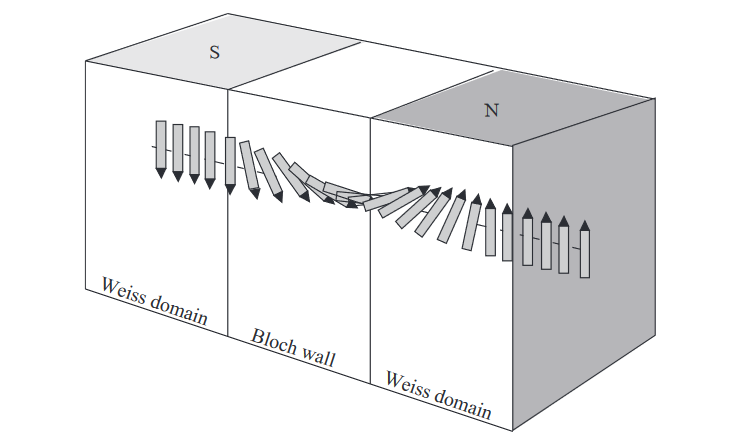
\includegraphics[width=0.35\textwidth]{domains_walls.png}
    \label{fig:domainsandwalls}
\end{figure}

Magnetization of a ferromagnetic material requires an  external magnetic field $H$.Two independent processes happen during the magnetization. These processes can be seen in Fig. \ref{fig:magnetization1}. 

First process is that at weak (relative to the levels of field required for other process) external fields, Bloch walls starts to move. This movement happens in such fashion that volume of Weiss domains which have the same magnetization direction as the external field starts to increase, and the volume of Weiss domains which have the opposite magnetization direction starts to decrease.

Other process is that at strong external fields, Weiss domains with magnetization direction normal to the external field are altered such that their magnetization direction starts to rotate towards the external field. This process requires such high external fields that, in some soft magnetic materials, Bloch wall movements are almost completed before the domain magnetization rotation happens.

Under the influence of an external fields low enough, Bloch walls only move slightly, and return back to their original position once the external field is removed. However, if higher external fields are applied, Bloch walls can not go back to their original position. This kind of Bloch wall displacement is called Barkhausen jumps. These jumps are irreversible, and they are the reason for ferromagnetic hysteresis.

In ferromagnetic materials, magnetization can be described in 3 phases. In first phase, only reversible Bloch wall motions occur. In second phase, Barkhausen jumps occur. In third phase, all the Weiss domains are magnetized in the direction of external field, and magnetic saturation settles. 





\begin{figure}[h]
    \centering
    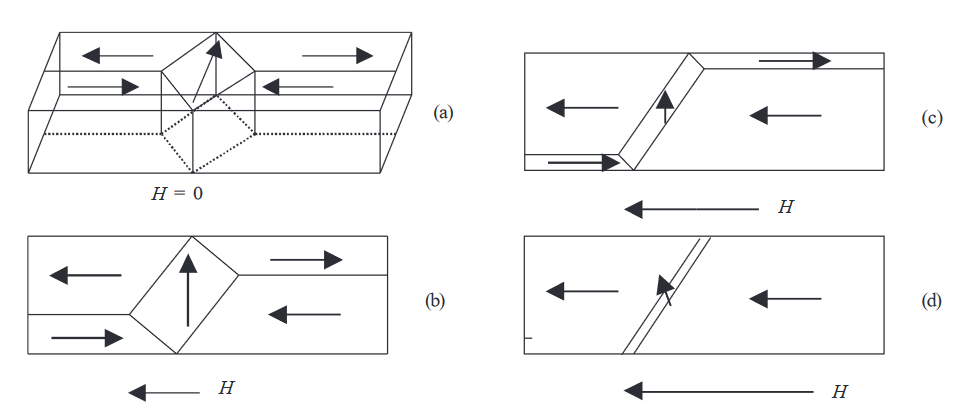
\includegraphics[width=0.85\textwidth]{magnetization1.png}
    \label{fig:magnetization1}
\end{figure}

\begin{figure}[h]
    \centering
    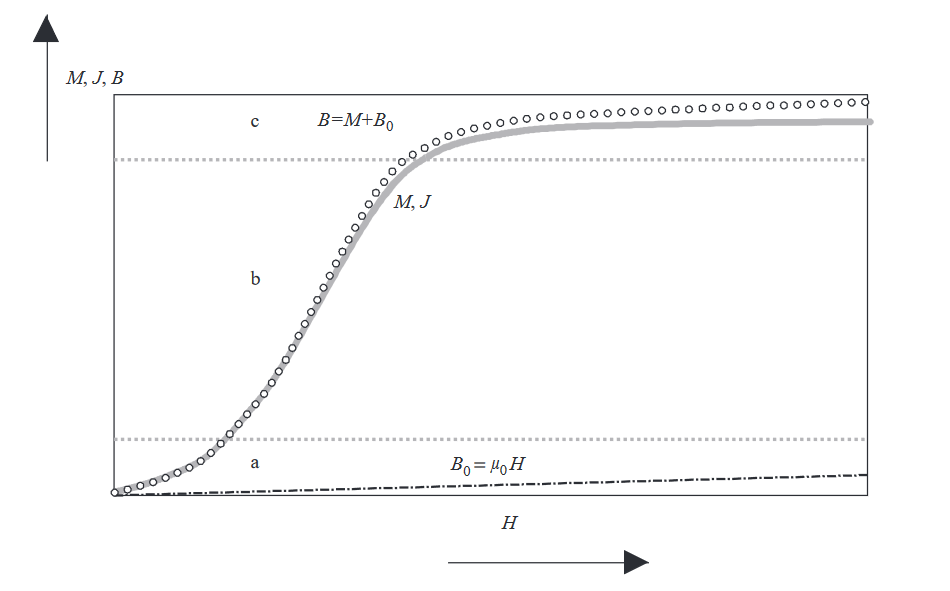
\includegraphics[width=0.35\textwidth]{magnetization2.png}
    \label{fig:magnetization2}
\end{figure}




\subsection{Losses in Iron Circuits: Pyrhonen 3.6.2}

\subsubsection{Hysteresis Losses}

\begin{equation}
	w_{1} = \int_{-B_{r}}^{B_{max}} HdB
\end{equation}



\begin{equation}
	w_{2} = \int_{B_{max}}^{B} HdB
\end{equation}

\begin{equation}
	W_{Hy} = V \oint HdB
\end{equation}

\begin{equation}
	P_{Hy} = f V w_{Hy}
\end{equation}
\begin{equation}
	P_{Hy} = \eta f V B_{max}^{k}
\end{equation}

\begin{figure}[h]
    \centering
    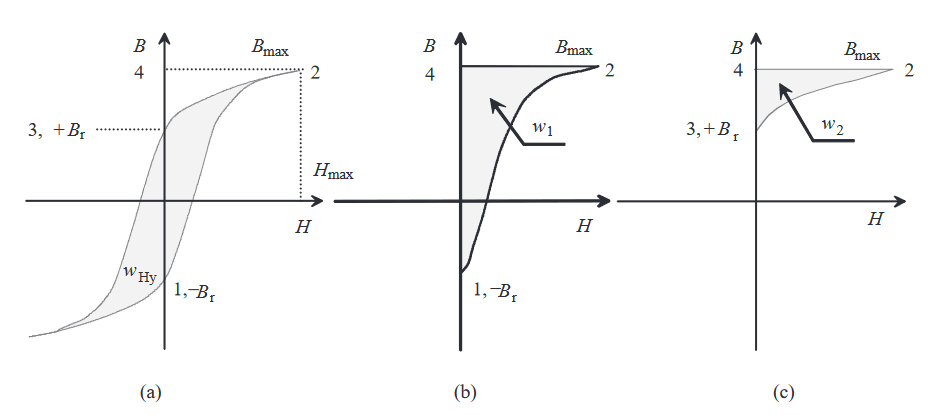
\includegraphics[width=0.35\textwidth]{hysteresiscurve1.png}
    \label{fig:hysteresiscurve1}
\end{figure}


\subsubsection{Eddy Current Losses}
Faraday's law states that alternating flux induces voltages. In a conductor, these induced voltages result with eddy current. The term 'eddy' comes from some analogy with fluid dynamics, and Leon Foucault is credited to be the one who discovered eddy currents.


\begin{equation}
	dI = \frac{E}{R} = \frac{2 \pi f \hat{B}_m w x dx}{\sqrt{2} \rho}
\end{equation}
\begin{equation}
	P_{Fe,Ft} = \frac{wh \pi^{2} f^{2} d^{3} \hat{B}_{m}^{2}}{6 \rho} = \frac{V \pi^{2} f^{2} d^{2} \hat{B}_{m}^{2}}{6 \rho}
\end{equation}

\section{Permanent Magnets in Rotating Machines: Pyrhonen 3.7}



\subsection{Operating Point of a Permanent Magnet Circuit: Pyrhonen 3.7.3}

To examine the operating point of a permanent magnet circuit, lets consider a permanent magnet material in the shape of a closed ring. The material is magnetized to saturation.


\paragraph{Magnetization:} a copper wire may be wound around the ring to form 1000 turns. Then, Ampere's law, Eq. \ref{eq:AmperesLaw} states:

\begin{equation}
	\oint \textbf{H} \cdot d\textbf{l} = NI = H 2\pi R
\end{equation}

if the ring has a radius of $R=10$ cm, then the current needed to supply $600$ kA/m is

\begin{equation}
	I = \frac{H 2\pi R}{N} = \frac{600,000 \times 2\pi \times 10 \times 10^{-3}}{1000}=37.7A
\end{equation}


The magnetizing equipment is removed. Now, as the external field is removed, PM supplies the remanent flux density $B = B_{r}$ at zero field $H=0$. At this moment, the operating point is on magnetic flux (induction) axis.

\paragraph{Magnetic Circuit: PM + Air gap}

A section of the ring is cut out, as depicted in Fig. \ref{fig:ringMagCirc}. If Ampere's law, Eq. \ref{eq:AmperesLaw} is again applied,

\begin{equation}
	\oint \textbf{H} \cdot d\textbf{l} = H_{PM}h_{PM}+H_{\delta}\delta = 0
	\label{eq:Ampereslaw_magcircapp}
\end{equation}

because there is no current enclosed by the ring, $\int_{A} \textbf{J} \cdot d\textbf{A}=0$. As the airgap length increases, demagnetizing field $H$ increases; therefore, PM magnetic flux density decreases. The slope of the load line increases and it's interception with the recoil curve, i.e. the operating point, moves towards left.
\begin{figure}[h]
    \centering
    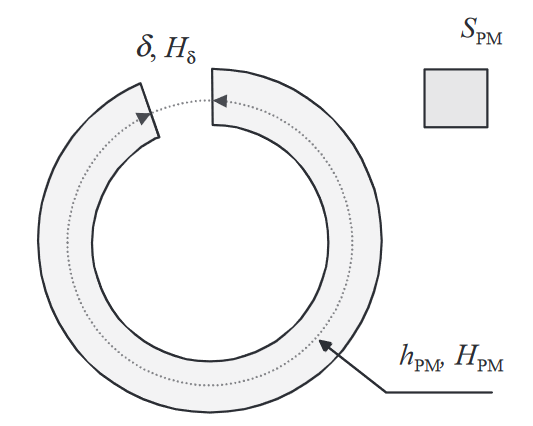
\includegraphics[width=0.45\textwidth]{ringMagCirc.png}
    \label{fig:ringMagCirc}
\end{figure}

\paragraph{Magnetic Circuit: PM + Air gap + Load} a coil is wound around the magnetic circuit. It is loaded with current $I$. The magnetic field path $d\textbf{l}$ encloses $N$ conductors, all of which carry a current $I$. Therefore, $\int_{A} \textbf{J} \cdot d\textbf{A} = \pm NI$. As a result, Ampere's Law is applied to the system as follows.

\begin{equation}
	\oint \textbf{H} \cdot d\textbf{l} = H_{PM}h_{PM}+H_{\delta}\delta = \pm NI
	\label{eq:Ampereslaw_magcircapp1}
\end{equation}

where $N$ is coil number of turns. The $\pm$ sign depends on the coil winding.

Loading the coil with current does not change the slope of the load line, but moves the line horizontally. If the magnetic field generated by the coil opposes the PM magnetic flux density, i.e. is in the same direction as PM demagnetizing field, then the load line, and therefore the operating point, moves to left. As a result, the operating point moves left as well. In contrast to this, if the coil is wound such that it's magnetic field is in the same direction as the PM magnetic flux density, i.e. opposes the PM demagnetizing field, then the load line, and therefore the operating point, moves to right.

As long as the operating point stays on the right side of the knee point, the resulting demagnetization is reversible, meaning that as the demagnetizing field on the PM fades, the PM again supplies it's original remanent magnetic flux density $B_{r}$. This can be called as partial reversible demagnetization. If the demagnetizing field increases too much,the operating point surpasses the knee. After this, the PM irreversibly loses some fraction of its magnetization, and the recoil curve declines to a position lower than the original recoil curve. This is called partial irreversible demagnetization. To achieve the original remanent magnetic field $B_{r}$, the PM needs to be magnetized again.

The recoil curve is not exactly straight. Therefore, even though the operation along the recoil curve is reversible, the operation itself incorporates hysteresis losses. A mere representation of this is depicted in Fig. \ref{fig:BHcurve1}. However, PM hysteresis losses are scarce and insignificant during normal operation in rotating electric machines \cite{pyrhonen_design_2014}.

\begin{figure}[h]
    \centering
    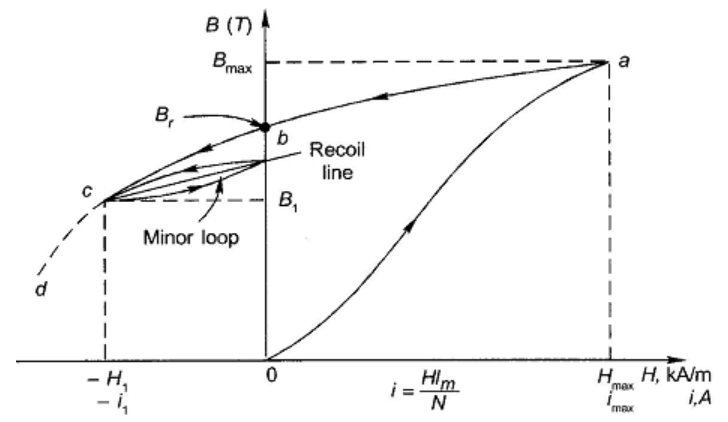
\includegraphics[width=0.70\textwidth]{BHcurve1.png}
    \label{fig:BHcurve1}
\end{figure}

  
\paragraph{Magnetic Circuit: PM + Soft Magnetic Material + Airgap}

Permanent magnets are expensive materials and they require intricate work to forge. Therefore, PMs are usually utilized with soft magnetic materials in applications. One such application and the resulting magnetic circuit is given in Fig. \ref{fig:softHardMagCirc}

\begin{figure}[h]
    \centering
    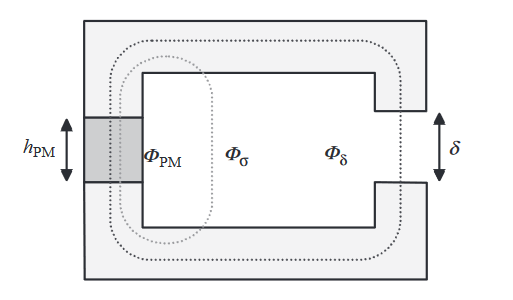
\includegraphics[width=0.45\textwidth]{softHardMagCirc.png}
    \label{fig:softHardMagCirc}
\end{figure}

Leakage flux and air gap flux are originated from the magnetic flux supplied by the PM. The permeance of the path with the air gap is much higher than the path of the leakage flux. Therefore,

PM sources the magnetic flux in this system. The path that consists of the soft magnetic material and the air gap is the path with the highest permeance. Therefore, majority of the magnetic flux travels through the air gap. Remaining small fraction of magnetic flux that does not travel through the air gap is called leakage flux.

The optimum operating point of a PM is at which the energy product $|BH|$ is at maximum. 


\paragraph{Magnetic Circuit Representation of PM}



\subsection{Demagnetization of Permanent Magnets: Pyrhonen 3.7.4}

There are 2 major reasons the operating point of a PM may pass the knee and demagnetize: the load is too high, or the temperature is too high.

\paragraph{Load Based Demagnetization}
Demagnetization happens if the operating point of the PM is on the nonlinear part of the B-H curve at second quadrant. PM temperature and the magnetic field intensity on the PM are 2 major actors in PM demagnetization process.




B-H curve for NdFeB magnet VACODYM 677TP can be seen in Fig. \ref{fig:vac677TP}. As can be seen, $-1000$ kA/m on this PM, at $20^{\circ}$ does no irreversible 

\paragraph{Temperature Based Demagnetization}




